\documentclass[12pt,a4paper,oneside]{report}

% Page layout
\usepackage[a4paper,top=1.7cm,bottom=7.4cm,left=2.5cm,right=6.0cm,footskip=6.3cm]{geometry}
\usepackage{setspace}
\usepackage{titlesec}
\titleformat{\chapter}[display]
  {\normalfont\huge\bfseries}{\thechapter}{20pt}{\Huge}
% Remove the "Chapter" word
\titleformat{\chapter}[display]
  {\normalfont\huge\bfseries}{}{0pt}{\Huge}
\usepackage{titling}
% Font setup for Arial-like appearance with pdfLaTeX
\usepackage[scaled=.92]{helvet} % Use Helvetica (closest to Arial for pdfLaTeX), scaled to match Arial proportions
\renewcommand{\familydefault}{\sfdefault} % Set sans-serif as default
\usepackage{algorithm}
\usepackage[noend]{algpseudocode}
\usepackage{threeparttable}
\usepackage{tabularx}
\usepackage{float}
\usepackage{multirow}
\usepackage{booktabs}
\usepackage{threeparttable}
\usepackage{adjustbox}
\usepackage{pdflscape}
% Include PDF
\usepackage{pdfpages}
% Bibliography - numbered citations with square brackets
\usepackage[numbers,square,sort&compress]{natbib}
\usepackage{fancyhdr}
\pagestyle{fancy}
\fancyhf{}
\fancyfoot[C]{\thepage}
\renewcommand{\headrulewidth}{0pt}
\renewcommand{\footrulewidth}{0pt}



\usepackage{url}
\usepackage{hyperref}
% Unicode support for pdfLaTeX
\usepackage[utf8]{inputenc}
\usepackage[T1]{fontenc}
% math
\usepackage{amsmath}

% for Plant Count section
\usepackage{tabularx}         % For tabularx environment
\usepackage{float}            % For H float option
\usepackage{subfig}           % For subfloat command
\usepackage{changepage}       % For adjustwidth environment
\usepackage{booktabs}         % For toprule, midrule, bottomrule commands
\usepackage{cleveref}         % For \cref command


% Paragraph formatting
\setlength{\parskip}{6pt}
\setlength{\parindent}{0pt}
\setstretch{1.5}

% Define extralength parameter
\newlength{\extralength}
\setlength{\extralength}{0cm}

\begin{document}

% Include the first page from the PDF file

\includepdf[pages=1]{Intestazione/t3._Thesis_first_page.pdf}

\abstract{

\textbf{Background and Research Gap:} Agricultural research for Plant 
Protection Product (PPP) development relies on statistical hypothesis testing. 
The European and Mediterranean Plant Protection Organizzation (EPPO) sets the 
standards for conducting tests in all its member countries. Traditional
statistical approaches recognised by EPPO address environmental variability through
experimental design features such as randomised controls. These methods require 
experimentalists to identify sources of environmental variability prior to data 
collection. This a priori identification of variance sources relies heavily on 
the expertise of the experimentalist rather than on systematic statistical 
procedures, which creates a significant limitation in agricultural field studies. 
Geostatistical methods offer an alternative approach, enabling the estimation of 
spatial environmental variability after data collection through variograms or 
spline fitting techniques. These methods are recognised by EPPO, but require 
spatially referenced data collection.

\textbf{Research Objectives:} With reference to the above-mentioned 
geostatistical approach, this research investigates the applicability of 
geomatics technologies for generating spatially referenced datasets across 
all EPPO-recognized observation categories, with the goal of demonstrating how 
these techniques can facilitate the adoption of geostatistical methods in 
hypothesis testing for agricultural research within the EPPO standard framework.

\textbf{Methodology:} 
This work considered three aspects of geomatics technologies applicability in 
this context:
\begin{enumerate}
\item counting, using deep learning object detectors to count maize seedlings on orthomosaics;
\item scoring, using machine learning regressors to score phytotoxicity via photogrammetric multispectral imaging and custom feature extraction;
\item classify, using anomaly detection to classify healthy or deseased plant tissues via pre-trained models.
\end{enumerate}

\textbf{Key Results:} To achieve EPPO benchmark performance ($R^2$ > 0.85) in 
maize seedling counting from orthomosaics, transformer-based object detectors 
required approximately 60 labeled training images ($225 \times 225$ pixels at 
$5\,\text{mm}/\text{pixel}$ resolution), with domain-specific training data 
proving essential for agricultural applications. Machine learning successfully 
automated phytotoxicity scoring ($\kappa$ > 0.7) with only 30 training samples 
by combining photogrammetric 3D models with spectral imaging, converting 
subjective ordinal assessments into objective continuous measurements suitable 
for enhanced statistical analysis. 
Pre-trained models achieved accurate plant deseases classification (accuracy > 0.85) 
using anomaly detection techniques without requiring task-specific training. 
All three approaches successfully demonstrated the feasibility of automatically 
collecting georeferenced observations for agricultural trial assessments that 
comply with EPPO standards, thereby enabling the implementation of geostatistical 
methods for improved spatial analysis.

\textbf{Novel Contribution:} This work establishes the first systematic 
evaluation of minimum requirements for implementing geomatics techniques within 
EPPO standards, providing practical guidelines for dataset size, validation 
protocols, and integration strategies. The research demonstrates that geomatics 
technologies can successfully provide spatial coordinates alongside observations 
for all EPPO variable types, enabling the implementation of geostatistical 
methods that improve environmental variability modeling compared to traditional 
experimental design approaches.

\textbf{Practical Impact:} The findings enable agricultural researchers to adopt 
more robust statistical methods for PPP trials by providing clear implementation 
requirements for digital data collection technologies, ultimately leading to more 
accurate efficacy evaluations and improved crop protection strategies.}

\clearpage

% Table of Contents
\tableofcontents
\newpage

% Main content
\chapter{Introduction}

\section{Research Overview and Motivation}

Agricultural research for plant protection product (PPP) development relies heavily 
on statistical hypothesis testing to establish efficacy and safety. Traditional 
experimental approaches in this field face a fundamental limitation: they 
require experimentalists to identify and control for environmental variability 
before data collection through experimental design features like randomized 
controls and blocking strategies. This "a priori" identification of variance 
sources depends heavily on experimentalist expertise and field experience 
rather than systematic statistical procedures, creating potential biases and 
limitations in agricultural field studies.

The European and Mediterranean Plant Protection Organization (EPPO) has 
established comprehensive standards for PPP evaluation that require rigorous 
statistical validation across diverse data types. However, classic statistical 
frameworks within these standards struggle to adequately address unknown spatial 
environmental variability that emerges during trials.

Geostatistical methods provide a well-established alternative approach, enabling 
the estimation of spatial environmental variability through mathematical 
techniques such as variograms and spline fitting. 
This approach fundamentally shifts the traditional paradigm by eliminating the 
need to have prior knowledge of environmental variability before starting the 
field trial. Instead, it enables this variability to be estimated afterwards, 
even when its effects overlap or interact with those of the treatments. While 
this analysis capability represents a significant advantage over classical 
experimental design approaches, geostatistics requires spatially referenced data 
collection, introducing the practical challenge of precise observation 
geolocation in agricultural field conditions.

Recent advances in geomatics technologies - including photogrammetry, spectral 
imaging, and machine learning - present new opportunities to overcome these 
limitations by providing efficient methods for generating spatially referenced 
datasets. However, the practical implementation of these technologies within the 
regulatory framework of PPP evaluation remains unexplored.

\section{Research Objectives}

This research investigates the applicability of geomatics technologies for 
recording spatially referenced observations across all EPPO standard categories. 
The overarching goal is to demonstrate how these technologies can facilitate the 
adoption of geostatistical methods in hypothesis testing for agricultural 
research conducted within the EPPO framework.

During my doctoral work, I categorized EPPO standard assessments into three main 
types of variables: continuous or discrete, ordinal, and nominal or binary. I 
selected one representative EPPO assessment for each variable type:

\begin{enumerate}
\item Plant counting (continuous or discrete)
\item Phytotoxicity scoring (ordinal)
\item Disease detection (nominal or binary)
\end{enumerate}

Each of these assessments was addressed through the application of geomatics 
technologies to demonstrate the feasibility of collecting georeferenced 
observations with precision and accuracy that meet EPPO standard requirements.

\section{Thesis Structure}

The structure of the thesis is as follows:

\textbf{Theoretical Background and Methodology} presents the theoretical 
foundation, including an overview of Plant Protection Product (PPP) regulations, 
relevant EPPO standards, and the methodological background covering geostatistics, 
photogrammetry, spectral imaging, and machine learning techniques.

\textbf{Applications Demonstration} presents three practical applications of 
geomatics technologies in recording georeferenced EPPO standard assessments:
\begin{itemize}
    \item \textbf{Continuous and Discrete Variables}: Investigation of minimum 
    dataset requirements for object detection in plant counting ("On the Minimum 
    Dataset Requirements for Fine-Tuning an
    Object Detector for Arable Crop Plant Counting: A Case Study on Maize 
    Seedlings" published in MDPI Remote Sensing, DOI: 10.3390/rs17132190)
    \item \textbf{Ordinal Variables}: Evaluation of machine learning approaches 
    for phytotoxicity scoring automation ("Supporting Screening of New Plant 
    Protection Products through a Multispectral Photogrammetric Approach 
    Integrated with AI" published in MDPI Agronomy, 
    DOI: 10.3390/agronomy14020306)  
    \item \textbf{Binary and Nominal Variables}: Application of anomaly 
    detection techniques for plant deseases unsupervised classification 
    (initial version of scientific paper still to be submitted). 
\end{itemize}

\textbf{Conclusions} summarise the main findings and discuss practical 
considerations for integrating geomatics technologies into PPP evaluation 
protocols.

\section{Literature Review and Research Gap}

\subsection{Current Limitations in Agricultural Statistical Design}

Traditional statistical analysis for PPP trials relies on Fisher's principles of experimental design \cite{fisherStatisticalMethodsResearch1992,meadStatisticalPrinciplesDesign2012,caslerFundamentalsExperimentalDesign2015}, which emphasize randomization, replication, and blocking to ensure validity of results. While this approach is well-established, it faces significant limitations in agricultural field studies where environmental heterogeneity is often unknown and difficult to predict \cite{paroliniPursuitScienceAgriculture2015,berryResistedRiseRandomisation2015}.

The experimental design components that most heavily rely on human judgment are block disposal and control arrangement \cite{tocherDesignAnalysisBlock1952,williamsOptimalityContrastsBlock2015}. Block disposal should minimize environmental variability within blocks while maximizing it between blocks \cite{vanesSpatialNatureRandomization1993,brienMultiphaseExperimentsLeast2011}, while control arrangement ensures untreated controls are not influenced by adjacent treated plots \cite{piephoWhyRandomizeAgricultural2013}.

Problems arise when unobserved environmental variability effects invalidate parametric statistical analysis due to heteroscedasticity of residuals \cite{schabenbergerStatisticalMethodsSpatial2004,onofriNewMethodAnalysis2010}. Shifting to non-parametric tests often results in decreased statistical power \cite{stroupRethinkingAnalysisNonNormal2015,agrestiIntroductionCategoricalData2018}.

\subsection{Geostatistical Approaches in Agricultural Research}

Geostatistical methods offer the potential to capture environmental variability "a posteriori" rather than requiring its prediction "a priori" \cite{oliverGeostatisticalApplicationsPrecision2010,websterGeostatisticsEnvironmentalScientists2007}. This approach should result in more robust and reliable statistical analysis, free from unexpected heterogeneity within experimental blocks \cite{richterGeostatisticalModelsAgricultural2012,lopezEfficiencyIncompleteBlock1995}.

Several studies have demonstrated the effectiveness of spatial variability estimation through geostatistical approaches \cite{bullockDataIntensiveFarmManagement2019,castrignanoGeostatisticalApproachModelling2017,jinEfficientGeostatisticalAnalysis2021,puntelLeveragingDigitalAgriculture2024,trevisanSpatialVariabilityCrop2021}. However, these approaches require georeferenced observations, which are often impractical for traditional visual assessments.

\subsection{Digital Technologies in Agricultural Assessment}

EPPO has recognized the potential of digital technologies through the publication of PP 1/333(1) \cite{PP1333}, which provides guidelines for incorporating digital tools into PPP trials. This standard requires that digital data meet the same quality standards as manual assessments, with specific validation benchmarks depending on variable type:

\begin{itemize}
    \item \textbf{Continuous and Discrete variables}: Coefficient of determination ($R^2$) > 0.85
    \item \textbf{Ordinal and Nominal variables}: Cohen's kappa coefficient ($\kappa$) > 0.7  
    \item \textbf{Binary variables}: Accuracy > 0.85
\end{itemize}

Recent advances in machine learning and computer vision have shown promise for automating agricultural assessments \cite{mahleinPlantDiseaseDetection2016,kamilarisDeepLearningAgriculture2018}, particularly when combined with photogrammetric and spectral imaging techniques.

\subsection{Research Gap and Innovation}

Despite the clear benefits of integrating geostatistics into PPP efficacy trials, the requirement for spatial coordinates alongside observations remains a significant barrier to widespread adoption. While modern technologies, toghether with geomatics techniques can provide spatial coordinates along with observations, systematic evaluation of their implementation requirements within the EPPO framework has not been conducted.

This research addresses this gap by investigating the minimum requirements needed to effectively produce georeferenced observations during efficacy trials, enabling the use of geostatistical methods to separate environmental variability from treatment effects in statistical analyses of PPP trials conducted under EPPO standards.

\chapter{Theoretical Background and Methodology}

\section{Regulatory Framework}

\subsection{PPPs and EPPO Standards}
PPPs are designed primarily to maintain crop health 
and prevent destruction by diseases and infestations. While the term "pesticides" 
is broader and also includes biocidal products used to control harmful organisms 
and disease carriers not related to plant protection, PPPs are 
specifically used to control harmful organisms affecting cultivated plants (such 
as insects, mites, fungi, bacteria, rodents, etc.), eliminate weeds, and regulate 
plant physiological processes. Fertilizers, which serve for plant nutrition and 
soil fertility improvement, are excluded from PPPs.

PPPs contain at least one active substance, which can be either 
chemical compounds or microorganisms, including viruses, that enable the product 
to perform its intended function. These active substances undergo rigorous risk 
assessment processes, with EFSA (European Food Safety Authority) playing a central 
role in conducting peer reviews at the EU level to determine if these products, 
when used correctly, might produce harmful effects on human or animal health, either 
directly or indirectly through drinking water, food, or feed.

The main categories of PPPs can be distinguished based on the 
type of organism they target or the function they perform, including:

\begin{itemize}
    \item Fungicides
    \item Insecticides
    \item Acaricides
    \item Nematicides
    \item Herbicides
    \item Plant growth regulators
\end{itemize}

The parameters identified through the risk assessment are compared with the values 
established by directive 97/57/EC \cite{EURLex1997265}, which indicates the acceptability limits for 
decision-making on the inclusion of active substances in the EU list (Annex I of 
directive 91/414/EEC \cite{directive_91_414_EEC}).

The Introduction of a product in the EU market is not only subject to audits on
active substances and their safety for humans and environment but also to the evaluation 
of the product's efficacy and safety for the crop.
World Trade Organization Sanitary and Phytosanitary Measures Agreement \cite{WTO_SPS_Agreement}
recognizes the International Plant Protection Convention (IPPC) as the only international
institution in charge of emitting standards for plant health \cite{IPPC}. IPPC is organized in
regions. European Union (EU) countries refer to the European and Mediterranean Plant
Protection Organization (EPPO). EPPO Standards are divided into Standards on
Phytosanitary Measures and Standards on PPPs. PPPs standards describe the efficacy
evaluation of PPPs (PP 1) and good plant protection practices. EU Good Experimental
Practices (GEP) units provide
Biological Assessment Dossier (BAD) efficacy trials. GEP units are expected to follow
EPPO PP 1 to assess PPPs selectivity detecting phytotoxicity effects, and efficacy in the
complaint of Regulation (EC) No 1107/2009 of the European Parliament and Council \cite{EC_Regulation_1107_2009}.

\section{EPPO Standards}

Generics on efficacy assessments are reported in PP 1/181(5) \cite{EPPO_PP1_181}, which describes
herbicide, fungicide, bactericide, and insecticide efficacy on the target evaluation.
PP 1/135(4) \cite{EPPO_PP1_135} describes the selectivity assessment procedures, 
in other words: the standard phytotoxicity assessments of PPPs.
The PP 1/152 \cite{EPPO_PP1_152} standard describes the general principles for the
efficacy and selectivity evaluation of PPPs, in describing the standard experimental design.
Aside from the objectives of the study and the description of treatments, 
the PP 1/152 outlined that a comprehensive experimental design should include a description of:
\begin{itemize}
    \item \textbf{Type of Design}
    \item \textbf{Sampling Method and Measures Units}
    \item \textbf{Statistical Analysis Plan}
\end{itemize}

\subsection{Experimental Design}

EPPO "envisage trials in which the experimental
treatments are the ‘test product(s), reference product(s) and
untreated control, arranged in a suitable statistical design’" \cite{EPPO_PP1_152}.
The experimental design should be randomized, with replications and blocks, and
should include a sufficient number of plots to ensure the statistical power of the
analysis. The number of replications and blocks should be determined based on the
expected variability of the data and the desired level of statistical significance
in respect to control and reference treatments. The
randomization of treatments within blocks should be carried out using a suitable
randomization procedure to ensure that the treatments are assigned to plots in a
completely random manner. The key randomization used in PPP 
evaluations include:

\begin{itemize}
    \item \textbf{Completely Randomized Design (CRD)}: Treatments randomly assigned to 
          experimental units; statistically powerful but only suitable for homogeneous trial 
          areas where environmental variation is minimal.
          
    \item \textbf{Randomized Complete Block Design (RCBD)}: Groups plots into homogeneous 
          blocks with each treatment appearing once per block; controls for environmental 
          heterogeneity across the experimental area.
          
    \item \textbf{Split-Plot Design}: Used when one factor (e.g., cultivation equipment) 
          cannot be fully randomized; creates hierarchy with whole plots and subplots; 
          particularly useful when plot size or equipment constraints exist.
          
    \item \textbf{Systematic designs}: Non-randomized arrangements rarely suitable for 
          efficacy evaluations; may only be appropriate in special cases like varietal 
          trials on herbicide selectivity.
\end{itemize}

When designing PPP trials, the arrangement of untreated controls 
is critical for proper efficacy assessment. According to EPPO standards, the main 
purpose of untreated controls is to demonstrate adequate pest infestation, without 
which efficacy cannot be meaningfully evaluated. Four distinct arrangements for 
untreated controls exist:

\begin{itemize}
    \item \textbf{Included controls}: The most common approach, where control plots 
    have the same shape and size as treatment plots and are fully randomized within 
    the experimental design. This arrangement is essential when controls 
    will be used in statistical comparisons.
    
    \item \textbf{Imbricated controls}: Control plots are arranged systematically 
    within the trial (between blocks or between treated plots), potentially with 
    different dimensions than treatment plots. These observations are typically 
    not included in statistical analyses but ensure more homogeneous distribution 
    of untreated area effects.
    
    \item \textbf{Excluded controls}: Control plots are established outside the 
    main trial area but in similar environmental conditions. While replication is 
    not essential, it may be beneficial in heterogeneous environments. These observations 
    are generally excluded from statistical analyses.
    
    \item \textbf{Adjacent controls}: Each plot is divided into two subplots, with 
    one randomly selected to remain untreated. This approach is particularly valuable 
    in highly heterogeneous environments but requires specialized split-plot statistical 
    analysis.
\end{itemize}

The selection of control arrangement depends on several factors: whether the control 
will be included in statistical tests (requiring included controls), the degree 
of environmental heterogeneity (adjacent controls are preferred for high heterogeneity), 
and the potential for control plots to interfere with adjacent treatment plots (suggesting 
excluded controls when interference is likely).
The trials type design is critical for the success of the study, as it ensures
that the results are reliable, reproducible, and statistically valid.

\subsection{Sampling Method and Measures Units}

While defining the experimental units through the randomisation design choice,
The sampling method and the units of measurement must also be defined.
Target and crop-specific standards point out "mode of
assessment recording and measurements" fixing evaluation metrics in two ways:
countable (discrete values) and measurable (continuous values) effects which must be
expressed in absolute values, in other cases, frequency (incidence) and degree
(severity) should be estimated and reported as affected percentage of the individual (ex.
plant or plot) or as proportion within treatment and control expressed in percentage. As
specified by PP 1/152 \cite{EPPO_PP1_152}, classification by ranking (ordinal) and scoring (ordinal or
nominal) is also contemplated. In the case of estimation, rather than count or measure,
PP 1/152 reports "The observer should be trained to make the estimations and his
observations should be calibrated against a standard". Calibration compliance with
standards is ensured by GEP audits. Scoring and ranking scales examples are
published on specific standards or the same PP 1/152. The lack of specific scales lets
trial protocol authors define one inspired in range and intervals by the mentioned
examples or other well-established ones.
GEP units PP 1 assessments are produced by trained and experienced
agronomists or biologists by visual inspection or laboratory analysis. The technician
follows the trial protocol and related EPPO standards during assessment execution. The
technician is critical for accuracy, precision, and repeatability. Sensitivity is determined
by the trial protocol. It depends on expected differences and if a measure, a proportion,
or a scale is used. For instance, in PP 1/93(3) \cite{EPPO_PP1_93} "Efficacy evaluation of herbicides -
Weeds in cereals - Observation on the crop", phytotoxicity color modification could be
measured, or estimated as proportion in respect to the untreated, or scored in EPPO
scale as PP 1/135(4) reports, or a scientifically accepted score as the European Weed
Research Society phytotoxicity damage score \cite{EWRS_score} and other ones.
In general, data types must undergo the classification presented in Table \ref{tab:data_types}.

\begin{table}[ht]
\caption{Different modes of observation and types of variables}
\label{tab:data_types}
\centering
\begin{tabular}{|l|c|c|c|}
\hline
\textbf{Type of Variable} & \textbf{Measurement} & \textbf{Ranking} & \textbf{Scoring} \\
\hline
Binary & & & X \\
\hline
Nominal & & & X \\
\hline
Ordinal & & X & X \\
\hline
Discrete & X & & \\
\hline
Continuous limited & X & & \\
\hline
Continuous not limited & X & & \\
\hline
\end{tabular}
\end{table}

\subsection{Statistical Analysis}

While PP 1/152 \cite{EPPO_PP1_152} doesn't prescribe 
specific analyses for all situations, it emphasizes that analysis methods should 
align with the experimental design and data types collected. For quantitative 
variables (continuous or discrete), parametric methods based on Generalized 
Linear Models (GLM) are recommended, including ANOVA and regression approaches. 
For qualitative variables (bynary, ordinal or nominal), non-parametric methods are more 
appropriate. Parametric analysis assumes additivity of effects, homogeneity of variance, 
and normally distributed errors. When these assumptions aren't met, data transformations 
or alternative approaches become necessary.

Statistical tests, particularly F-tests of orthogonal 
contrasts, should focus on biologically relevant comparisons specified during the 
design stage: untreated control versus treatments (establishing trial validity), 
reference products versus control (demonstrating coherence), test products versus 
reference (evaluating efficacy), and comparisons among test products (identifying 
superior treatments). For efficacy trials, EPPO suggests one-sided tests since the 
aim is comparing products against references or controls, with appropriate multiple 
comparison procedures when needed.

In pragmatic undertakings, analyses with parametric models are frequently 
favoured over non-parametric ones because parametrics have greater statistical 
power for the same number of 
observations \cite{agresti_exact_2001}.
This often results in experiments being designed that use continuous or discrete 
variables instead of binary, nominal or ordinal ones. These continuous or 
discrete variables are often recorded through visual estimation rather than 
true measurements or counting because the latters are more time-consuming and require more 
equipment \cite{bockPhytopathometryGlossaryTwentyfirst2022,chiang_quantitative_2020,
moraes_characterizing_2022}. However, using visual estimates often results in 
fitting parametric models that violate key assumptions, such as normally 
distributed residuals and homoscedasticity 
\cite{stevenson_overview_2001,acutis_perfunctory_2012,chiang_what_2014}.
This can lead to unjustified transformations or the use of non-parametric models, resulting in a loss of statistical power.

\subsection{Geomatics Methods in EPPO Standards}

Through adherence to rigorous design, variables types and analysis standards, researchers can 
generate reliable evidence to support PPP registration while ensuring 
that products demonstrate consistent efficacy across relevant agricultural conditions.
Nevertheless, the traditional statistical approaches face significant limitations in
agricultural field studies where environmental heterogeneity is often unknown and
difficult to predict, or even when visual estimates are used to assess
variables that should be measured or counted.
This is where geostatistical methods
can provide a significant advantage by enabling post-hoc estimation of spatial
environmental variability.
The fundamental advantage of geomatics over traditional statistical approaches 
lies in its ability to agnostically capture spatial variability in a continuous dimension 
rather than predefined block and replication factors that rely on subjective experience. 
Traditional statistical analysis for PPP trials still relies on 
Fisher's principles of experimental design 
\cite{fisherStatisticalMethodsResearch1992,meadStatisticalPrinciplesDesign2012,caslerFundamentalsExperimentalDesign2015},
which emphasize the importance of randomization, replication, and blocking to 
ensure the validity of results. Even if this approach for the experimental design 
is well-established, it is not without weaknesses: it relies on the 
agronomist-experimentalist knowledge and experience of the field where the trial 
is performed that can be limited and biased as any human observation 
\cite{paroliniPursuitScienceAgriculture2015,berryResistedRiseRandomisation2015}. 
The experimental design part 
that mostly relies on human choice is the block/replication disposal and the experimental units 
arrangement \cite{tocherDesignAnalysisBlock1952,williamsOptimalityContrastsBlock2015}. 
The block and replication disposal 
should guarantee that the environmental variability is minimized within the block
and maximized between blocks \cite{vanesSpatialNatureRandomization1993,brienMultiphaseExperimentsLeast2011}, 
while 
the experimental units arrangement ensures that the treatments and untreated control are not influenced by 
adjacent treated plots \cite{piephoWhyRandomizeAgricultural2013}.
Problems arise when environmental variability effects, unobserved during set-up, 
make the parametric statistical analysis invalid due to heteroscedasticity of the 
residuals \cite{schabenbergerStatisticalMethodsSpatial2004,onofriNewMethodAnalysis2010}. 
Often in such cases, 
shifting to non-parametric tests could mean a decrease 
of power \cite{stroupRethinkingAnalysisNonNormal2015,agrestiIntroductionCategoricalData2018}
and often is not the final solution for biased trials.
If the experimental design and the statistical model could be able to catch 
the environmental variability "a posteriori" instead of guessing its distribution "a priori"
\cite{oliverGeostatisticalApplicationsPrecision2010,websterGeostatisticsEnvironmentalScientists2007}, 
the statistical analysis should be more robust, reliable and free from
unexpected heterogeneity within the blocks
\cite{richterGeostatisticalModelsAgricultural2012,lopezEfficiencyIncompleteBlock1995,aquiles_e_effect_2024}.

EPPO recognizes the application of geostatistical methods in agricultural 
experimentation recommending GLMs as the underlying 
model structure for ANOVA.
Geostatistical methods can be incorporated into Generalized Linear Mixed Models 
(GLMMs) to account for spatial variability arising from replication structures 
or pseudoreplication \cite{gburAnalysisGeneralizedLinear2020,kumleEstimatingPowerGeneralized2021}, 
thereby improving the accuracy of inferences and reducing 
Type I errors
\cite{slaets_linear_2021,millar_remedies_2004,Piepho_2011,schabenbergerStatisticalMethodsSpatial2004,aquiles_e_effect_2024}.
However, in order to apply geostatistical methods, experimental observations must 
be georeferenced, i.e. associated with spatial coordinates. This can increase 
field data acquisition time and the need for technological instrumentation 
(e.g. GPS, remote sensors or drones), affecting the logistical costs of 
experimentation \cite{antoniou_chapter_2023,alexopoulos_complementary_2023,zhao_grain_2011}.
Nevertheless, the evolution of automated digital surveying technologies, 
such as multispectral sensors mounted on UAVs, agricultural IoT devices and 
georeferenced mobile apps, is rapidly reducing the cost and complexity of 
georeferencing in experimental agriculture \cite{cisternas_systematic_2020,mondino_considerazioni_2017}.
Additionally, using real georeferenced measurements instead of subjective 
visual estimates reduces the risk of violating the assumptions of parametric 
statistical models (e.g. normality of residuals or homogeneity of variance) 
\cite{stevenson_overview_2001,acutis_perfunctory_2012,chiang_what_2014}.
Consequently, geostatistics can be a viable alternative to classical 
block-based statistics, offering greater robustness and statistical power, 
particularly in contexts of high spatial heterogeneity.

\section{Geomatics}

Geomatics is an integrated approach to the measurement, analysis, management, 
and display of geographically referenced information 
\cite{gomarascaBasicsGeomatics2009}.  
This research focus on two main aspects of geomatics: the acquisition of spatially 
referenced data and the application of geostatistical methods to analyze 
this data. Geomatics encompasses a range of technologies and techniques that 
enable precise spatial data acquisition, including georeferenced sensors, 
photogrammetry, spectral imaging, and machine learning. 
In agricultural research, georeferenced sensors integrated into machinery such 
as harvesters and sprayers are widely employed to collect spatially explicit 
data on crop yield, soil characteristics, and other agronomic parameters. 
These technologies are complemented by photogrammetry, which enables geometric 
reconstruction and the quantification of structural features from images; 
spectral imaging, which captures reflectance across multiple wavelengths to 
infer biological and physical attributes; and machine learning algorithms, 
which support automated measurement, score and rank. 
These techniques collectively provide the capability to generate 
spatially-referenced datasets essential for implementing geostatistical methods 
in PPP trials.

\subsection{Geostatistics}

Variograms are fundamental tools in geostatistics that quantify 
the spatial dependence of a random field 
\cite{cressieStatisticsSpatialData2015,goovaertsGeostatisticsNaturalResources1997}. 
They characterize how data similarity 
changes with distance, making possible to include the indipendent from the treatments
spatial variation in a parametric model. 
The empirical (sample) variogram $\hat{\gamma}(h)$ is calculated by:
\[
\hat{\gamma}(h) = \frac{1}{2|N(h)|} \sum_{(i,j) \in N(h)} [z(s_i) - z(s_j)]^2
\]

where $z(s_i)$ is the observed value at location $s_i$, $N(h)$ is the set of all 
point pairs separated by distance $h$, and $|N(h)|$ is the number of such pairs
\cite{matheronPrinciplesGeostatistics1963,journelMiningGeostatistics2003}.
Variogram estimation typically follows a two-step process: first calculating the 
empirical variogram from observed data points, then fitting a theoretical model to 
this empirical structure \cite{websterGeostatisticsEnvironmentalScientists2007, oliverGeostatisticalApplicationsPrecision2010}. 
The empirical variogram is influenced by several factors:

\begin{itemize} 
    \item \textbf{Lag distance}: The distance interval $h$ at which pairs of points are compared 
    \item \textbf{Binning}: How distance classes are discretized when calculating average semivariance 
    \item \textbf{Directional parameters}: Whether to consider anisotropy (directional dependence) 
    \item \textbf{Maximum distance}: The upper limit of separation distance to include 
\end{itemize}

Variogram parameters that require configuration, often without direct 
optimization so reling on statistician-agronomic knowledge
\cite{mullerGeostatisticalModellingPython2022}, 
include:

\begin{itemize} 
    \item \textbf{Nugget} ($c_0$): The y-intercept of the variogram, representing measurement error and microscale variation 
    \item \textbf{Sill} ($c$): The plateau value reached by the variogram, equal to the variance of the random field 
    \item \textbf{Range} ($a$): The distance beyond which observations become spatially independent 
    \item \textbf{Anisotropy ratio}: The ratio between the maximum and minimum ranges in different directions 
    \item \textbf{Anisotropy angle}: The direction of maximum spatial continuity 
\end{itemize}

Theoretical variogram models must be selected to fit the empirical variogram
\cite{cressieStatisticsSpatialData2015, goovaertsGeostatisticsNaturalResources1997}. 
Common models include:

\begin{itemize} 
    \item \textbf{Spherical model}: Exhibits a progressive decrease of spatial dependence until reaching the range 
    \item \textbf{Exponential model}: Approaches the sill asymptotically, with practical range typically defined at 95\% of the sill 
    \item \textbf{Gaussian model}: Shows a parabolic behavior near the origin, indicating high continuity 
    \item \textbf{Matérn model}: Offers flexibility through an additional smoothness parameter 
    \item \textbf{Power model}: Used for non-stationary processes without a finite variance 
    \item \textbf{Nugget effect model}: Represents microscale variation or measurement error 
\end{itemize}

Proper variogram modeling for excluding spatial variation in a parametric model
must be fitted on control samples \cite{larkOptimizedSpatialSampling2002, minasnyEfficiencyVariousApproaches2002,aquiles_e_effect_2024}
to avoid including treatment effects in the 
spatial terms of the parametric model. 
The control samples must be homogeneously distributed
in the space and also in time if the aim is to get spatiotemporal variation.
In order to ensure the right control sampling, it is necessary to implement a 
combined approach using both imbricated or adjacent controls along with included 
controls in the following manner:
imbricated or adjacent control observations to fit the variogram model 
while the included control to test the error of the variogram predictions in a
cross-validation fashon. Testing on included controls ensures the variogram model 
error estimates aren't biased by the spatial arrangement of control observations. 
Nevertheless, it is possible to not include control and test variogram model errors
through other cross-validation technics such as Leave-One-Out or K-Folds on the 
imbricated or adjacent controls
\cite{websterGeostatisticsEnvironmentalScientists2007,henglPracticalGuideGeostatistical2007}. 
If the only imbricated control is present, area size of control is even 
more important, because having it smaller than treatment plot size could lead to a 
wrong estimation of the variogram model. In practical terms, in an imbricated control
arrangement, a buffer area with width equal to the treatment plot width must be placed around each plot,
resulting equivalent to an adjacent control arrangement. 
The spatial varibility estimation through variogram modeling was already proved 
to be effective in many studies \cite{bullockDataIntensiveFarmManagement2019,castrignanoGeostatisticalApproachModelling2017,jinEfficientGeostatisticalAnalysis2021,puntelLeveragingDigitalAgriculture2024,trevisanSpatialVariabilityCrop2021}, 
but it has the drawback of requiring a large control area. 

If incorporating such large control areas is not feasible and only included 
controls are available, 
one can rely on Spatial Analysis of field Trials with Splines (SpATS)
\cite{rodriguez-alvarezCorrectingSpatialHeterogeneity2018,rodriguez-alvarezFastSmoothingParameter2015,leeEfficientTwodimensionalSmoothing2013}.
SpATS is a statistical model that enables correction of spatial heterogeneity
of the data by using splines to model the spatial trend of the response variable.
The SpATS model is based on the assumption that the response variable can be
described as a function of the treatment effects and a smooth spatial trend.
The model can be expressed as:
\[
y_{ij} = \mu + \tau_i + f(u_j, v_j) + \varepsilon_{ij}
\]

where: 
\begin{itemize} 
    \item $y_{ij}$ is the response variable observed at the $j$-th location for the $i$-th treatment 
    \item $\mu$ is the overall mean \item $\tau_i$ represents the fixed effect of the $i$-th treatment 
    \item $f(u_j, v_j)$ is the smooth spatial trend modeled using tensor-product P-splines, where $u_j$ and $v_j$ are the spatial coordinates of the $j$-th location 
    \item $\varepsilon_{ij}$ is the random error term, typically assumed to be normally distributed with zero mean and constant variance 
\end{itemize}

The spatial component $f(u_j, v_j)$ can be further decomposed into additive and 
interaction effects: 
\[
f(u_j, v_j) = f_1(u_j) + f_2(v_j) + f_{12}(u_j, v_j)
\]

where $f_1(u_j)$ and $f_2(v_j)$ are the main effects for rows and columns, 
and $f_{12}(u_j, v_j)$ represents the smooth interaction surface that accounts 
for localized spatial patterns. The smoothing parameters controlling the flexibility 
of these components are estimated using restricted maximum likelihood (REML).
According to Rodriguez-Alvarez et al. (2018) 
\cite{rodriguez-alvarezCorrectingSpatialHeterogeneity2018}, 
SpATS has been effectively applied 
to field trials with varying dimensions, but there are practical considerations 
for minimum requirements: a minimum grid of 5x5 (25 plots) is often considered a 
practical lower limit, but complex spatial variations might require a bigger grid.
SpATS has been successfully applied to breeding trials with experimental designs 
exceeding hundreds of rows and columns, whereas the variogram approach can be effective 
even with a single treatment plot, provided sufficient control area is available.
Thus, as a rule of thumb, for trials with sufficient space to implement imbricated
or adjacent checks with included control, variogram is advised,
while for trials with many individuals (at least more than 25 in a regular grid) 
and constrained space, SpATS estimations is often better.
To evaluate how effectively the fitted model describes spatial variability of the 
data for SpATS, 
residuals of included control repetitions (compared to their mean) should be 
smaller than the combined model random and unexplained variation.
For both approaches, finding the optimal model across parameters that cannot be 
directly solved requires, 
an iterative approach testing various settings can be deployed. 

All the described geostatistical techniques can be seamlessly integrated with GLMMs to
provide a comprehensive analysis of spatial-temporal data
\cite{slaetsLinearMixedModels2021,rodriguez-alvarezCorrectingSpatialHeterogeneity2018}, 
enhancing the accuracy and reliability of treatment effect estimates in orthogonal
tests.

\subsection{Geomatics Thecnics and Digital Technologies}

As already mentioned, the EPPO standards require that the
observations are made by trained experimentalists.
To regulate the use of technologies that can measure, rank or score instead of 
experimentalists, the EPPO published a new standard (PP 1/333(1)\cite{PP1333}) which 
addresses the use of digital technologies in PPP efficacy and selectivity trials.
This standard provides guidelines for incorporating digital
tools into trial protocols, where digital tools are intended as a combination of
hardwares and softwares delivering data 
in a semi-automatic or automatic fashon.
The digital data must respect the same quality standards of the manual
ones, and the digital tools must be validated before the trial execution.
Validation of digital tools should
be performed by comparing the results of digital and manual assessments, 
demonstrating that the digital tools provide reliable and consistent
results compared to manual assessments golden sample. 
The benchmarks for the validation depends
on the type of variable. For each type of variable, the congruence between 
digital and manual should be evaluated with a different metric:

\begin{itemize}
    \item \textbf{Continuous and Discrete}: Coefficient of determination ($R^2$) higher than 0.85.
    \item \textbf{Ordinal and Nominal}: Cohen's kappa Coefficient ($\kappa$) higher than 0.7.
    \item \textbf{Binary}: Accuracy higher than 0.85
\end{itemize}

The variable type also influence the kind of digital tool to use.
The hardware of a digital tool is always a sensor to collect the raw data and a
processor to convert the raw data in a digital format.
For what concerns the software of a digital tool, it is worth to mention that
the core of it is always a model that convert the digital format into the assessment
observation in the variable units.
Quantitative variables are produced by regression models, while qualitative (categorical) 
variables are produced by classification models. 
Quantitative variables: continuous (limited or not) and discrete
can be summarized as metric measurments and counts respectively.

The capability of digital tools to measure and georeference harvest-related 
parameters such as yield weight, moisture content, and hectolitric weight 
is well established \cite{cisternas_systematic_2020,zhao_grain_2011,mahleinHyperspectralSensorsImaging2018}. However, parameters that are more complex to assess 
digitally, including plant counts, phytotoxicity symptoms, and disease 
incidence or severity, have garnered significant research interest in 
recent decades \cite{bockSpecialIssuePhytopathometry2022,bockVisualEstimatesFully2020,bockPlantDiseaseSeverity2010,mahleinHyperspectralSensorsImaging2018}. 
Despite technological advancements, a definitive consensus has yet to emerge 
regarding the extent to which these tools can fully substitute for human 
observers \cite{barbedoAutomaticMethodDetect2014,bockVisualEstimatesFully2020,arnalbarbedoDigitalImageProcessing2013}. Nevertheless, their adoption undoubtedly enhances field assessments 
by incorporating georeferenced data, so enabling
geostatistics for efficacy trials.
This study aims to evaluate the potential of geomatics-based technologies for 
collecting observational data in agricultural trials conducted under EPPO 
standards. Specifically, it investigates the use of photogrammetry, 
spectral imaging, and machine learning as digital tools for capturing trial 
observations across all variable types recognized by EPPO guidelines.

\subsubsection{Photogrammetry}

Photogrammetry is a technique used to obtain reliable information about physical 
objects and the environment through the process of recording, measuring, and interpreting 
photographic images. It is widely used in various fields such as topographic mapping, 
architecture, engineering, manufacturing, quality control, and geology. The fundamental 
principle of photogrammetry is based on the geometry of image formation and the 
mathematical relationships between the images and the objects being photographed
\cite{hartleyMultipleViewGeometry2003,krausPhotogrammetryGeometryImages2007}.
The basic principle of photogrammetry involves capturing multiple photographs of 
an object or scene from different perspectives. By analyzing these images, it is 
possible to reconstruct the three-dimensional (3D) coordinates of points on the 
object's surface. The key steps in photogrammetry include image acquisition, image 
orientation, and 3D reconstruction
\cite{hartleyMultipleViewGeometry2003,szeliskiComputerVisionAlgorithms2022}.

Images are typically captured using cameras mounted on various platforms such as 
tripods, drones, or aircraft. The quality and resolution of the images are crucial 
for accurate photogrammetric analysis. The images should have sufficient overlap 
(usually 60-80\%) to ensure that common points are visible in multiple images
\cite{colominaUnmannedAerialSystems2014,nexUAV3DMapping2014}.

Image orientation involves determining the position and orientation of the camera 
at the time each photograph was taken. This process is divided into two main steps: 
interior orientation and exterior orientation 
\cite{brownCloseRangeCameraCalibration2002,triggsBundleAdjustmentModern2000}.

\begin{itemize}
    \item \textbf{Interior Orientation:} This step involves determining the internal 
    geometry of the camera, including the focal length, principal point, and lens 
    distortion parameters. These parameters are typically obtained through a camera 
    calibration process.
    \item \textbf{Exterior Orientation:} This step involves determining the position 
    (X, Y, Z coordinates) and orientation (roll, pitch, yaw angles) of the camera 
    in a global coordinate system. While tie points from overlapping images establish 
    relative orientation between images, absolute exterior orientation requires 
    Ground Control Points (GCPs) with known coordinates or other external reference 
    information (such as GNSS/IMU data) to establish the relationship between image 
    coordinates and real-world coordinates.
\end{itemize}

Once the images are oriented, the 3D coordinates of points on the object's surface 
can be reconstructed using triangulation. Triangulation is a mathematical process 
that involves intersecting lines of sight from multiple images to determine the 
precise location of a point in 3D space
\cite{hartleyMultipleViewGeometry2003,furukawaAccurateDenseRobust2010}.

Mathematically, the process can be described using the collinearity equations, which 
relate the image coordinates (x, y) of a point to its object coordinates (X, Y, Z) 
through the camera parameters
\cite{wolfElementsPhotogrammetryApplication2013,krausPhotogrammetryGeometryImages2007}:

\[
\begin{aligned}
    x &= x_0 - \frac{f \cdot (r_{11}(X - X_0) + r_{12}(Y - Y_0) + r_{13}(Z - Z_0))}{r_{31}(X - X_0) + r_{32}(Y - Y_0) + r_{33}(Z - Z_0)} \\
    y &= y_0 - \frac{f \cdot (r_{21}(X - X_0) + r_{22}(Y - Y_0) + r_{23}(Z - Z_0))}{r_{31}(X - X_0) + r_{32}(Y - Y_0) + r_{33}(Z - Z_0)}
\end{aligned}
\]

where:
\begin{itemize}
    \item \( (x_0, y_0) \) are the coordinates of the principal point in the image.
    \item \( f \) is the focal length of the camera.
    \item \( (X_0, Y_0, Z_0) \) are the coordinates of the camera position.
    \item \( r_{ij} \) are the elements of the rotation matrix that describes the orientation of the camera.
\end{itemize}

By solving these equations for multiple images, the 3D coordinates of the object 
points can be accurately determined.
Recognized object points can be more or less sparse depending on the approach to 
their recognition and pairing. 
Historically, homologous points within images was
performed manually. Today many algorithms for this task are available. 
They can be divided between point-based and area-based algorithms.
Point-based algorithms identify and match distinct points in the images, such as
corners or edges. These algorithms rely on feature descriptors (e.g., SIFT, SURF, ORB)
\cite{loweDistinctiveImageFeatures2004,baySpeededUpRobustFeatures2008,rubleeORBEfficientAlternative2011}
to extract and match key points across images. Area-based algorithms, on the other hand,
use the entire image region to find correspondences. They typically involve
template matching or correlation techniques to identify similar regions in different images.
The choice of algorithm depends on the specific application and the characteristics
of the images being processed.
The 3D reconstruction process can also be enhanced using additional techniques such as
structure from motion (SfM) and multi-view stereo (MVS)
\cite{westobyStructurefromMotionPhotogrammetryLowcost2012,seitzComparisonEvaluationMultiView2006}. 
SfM is a technique that
estimates the camera motion and 3D structure of a scene simultaneously from a
set of images. It involves detecting and matching feature points across multiple images,
and then using these correspondences to estimate the camera parameters and the 3D
coordinates of the points. MVS, on the other hand, focuses on dense reconstruction
by estimating the depth information for each pixel in the images. It uses the camera
parameters and the matched feature points to create a dense point cloud or a 3D mesh
of the scene.
The resulting 3D model can be visualized and analyzed using specialized software,
allowing for measurements of distances, areas, and volumes. Photogrammetry can also
be used to create orthophotos, which are geometrically corrected images that can be
used for mapping and analysis
\cite{mikhailIntroductionModernPhotogrammetry2001,paineAerialPhotographyImage2012}. 
Orthophotos are generated by removing the effects of
perspective distortion and terrain relief from the original images, resulting in a
scale-accurate representation of the area.

\subsubsection{Spectral Imaging}
Spectral imaging is a technique that captures images at multiple wavelengths
of the electromagnetic spectrum, providing valuable information about the spectral
characteristics of objects and materials
\cite{meerImagingSpectrometryBasic2001,thenkabailHyperspectralRemoteSensing2016}. 
Multispectral images are typically acquired using specialized
cameras or sensors that can capture light in different spectral bands, ranging
from ultraviolet (UV) to infrared (IR) wavelengths
\cite{thenkabailHyperspectralRemoteSensing2016,mahleinHyperspectralSensorsImaging2018}. 
Some study tested also the 
feasibility to use bands in the termal infrared (TIR) range \cite{wanOptimizingUAVbasedUncooled2024}.
Each spectral band corresponds
to a specific range of wavelengths, allowing for the analysis of the spectral
signature of objects in the scene.
The spectral signature is the unique pattern of reflectance or absorption of
light at different wavelengths for a specific material or object. By analyzing
the spectral signatures of different materials, it is possible to identify and
classify them based on their spectral characteristics. This is particularly useful
in applications such as vegetation analysis, where different plant species exhibit
distinct spectral signatures due to variations in leaf pigments, moisture content,
and other physiological factors
\cite{sarviaGeometricVsSpectral2024}.
Multispectral imaging can be performed using various platforms, including
drones, satellites, and ground-based systems. The choice of platform depends on
the specific application, the spatial resolution required, and the area of interest.
The images captured by multispectral sensors are typically processed using
specialized software that applies various algorithms to extract relevant information
from the spectral data. This processing may include radiometric correction,
geometric correction, and atmospheric correction to ensure accurate and reliable
results.
The resulting multispectral images can be analyzed to derive various indices
and metrics that provide insights into the health and condition of vegetation.
One of the most commonly used indices in agriculture is the Normalized Difference
Vegetation Index (NDVI), which is calculated using the red and near-infrared
(NIR) bands of the multispectral image \cite{rouseMonitoringVegetationSystems1974,tuckerRedPhotographicInfrared1979}. 
NDVI is a measure of vegetation
greenness and is widely used to assess plant health, monitor crop growth, and
detect stress conditions. The NDVI is calculated using the following formula:
\[
NDVI = \frac{NIR - Red}{NIR + Red}
\]
where \(NIR\) and \(Red\) are the reflectance values in the near-infrared and red
bands, respectively. NDVI values range from -1 to +1, with higher values indicating
greater vegetation density and health. NDVI is particularly useful for monitoring
crop growth, assessing drought conditions, and detecting plant diseases.
Other indices derived from multispectral images include the Enhanced
Vegetation Index (EVI), Soil-Adjusted Vegetation Index (SAVI), and Leaf Area
Index (LAI), each providing specific information about vegetation health and
condition
\cite{hueteOverviewRadiometricBiophysical2002,qiModifiedSoilAdjusted1994}. 
These indices can be used to monitor crop performance, assess
nutrient status, and evaluate the impact of environmental factors on plant
growth
\cite{jonesRemoteSensingVegetation2010,mahleinHyperspectralSensorsImaging2018}

\subsubsection{Machine Learning}

Machine Learning (ML) is a branch of artificial intelligence (AI) that 
focuses on the development of algorithms and models capable of learning 
from and making predictions or decisions based on data \cite{kozaAutomatedDesignBoth1996}. 
Unlike traditional 
programming, where explicit instructions dictate the output for given inputs, 
ML models identify patterns and relationships within data to generate 
predictive outcomes \cite{hastieElementsStatisticalLearning2009}. 
These techniques are particularly valuable when 
dealing with large, complex, or high-dimensional datasets, where manual 
analysis would be impractical or inefficient.

ML has gained substantial importance in various scientific fields, including 
agriculture \cite{araujoMachineLearningApplications2023} and 
plant protection \cite{bockVisualEstimatesFully2020}. 
Within the context of PPP 
efficacy evaluation, ML offers new opportunities to enhance data processing, 
interpretation, and decision-making by leveraging vast amounts of observational 
data collected during field trials \cite{bockSpecialIssuePhytopathometry2022}. Integrating ML approaches into the framework 
of PP1/333 can significantly increase the robustness and accuracy of the analysis, 
allowing for more data-driven and automated assessments 
\cite{barbedoAutomaticMethodDetect2014,arnalbarbedoDigitalImageProcessing2013,bockPlantDiseaseSeverity2010}.

The primary objective of employing ML techniques in PPP trials 
is to improve accuracy, precision, and reproducibility while reducing manual 
intervention and subjective bias \cite{bockVisualEstimatesFully2020}. Modern ML methods can analyze complex interactions 
between variables and predict treatment outcomes under various conditions, thereby 
facilitating more efficient and accurate efficacy assessments.

There are several fundamental approaches in machine learning, each suited to different 
types of tasks and data structures:

\begin{itemize}
    \item \textbf{Supervised Learning}: Models are trained on labeled datasets where 
    the input-output relationship is known. Techniques include regression, classification, 
    and ensemble methods such as Random Forests and Gradient Boosting.
    \item \textbf{Unsupervised Learning}: Models identify patterns or groupings within 
    data without labeled responses. Clustering (e.g., K-means, hierarchical clustering) 
    and dimensionality reduction (e.g., PCA, t-SNE) are common techniques.
    \item \textbf{Weakly-supervised Learning}: Combines a small amount of labeled data with 
    a large amount of unlabeled data to improve learning accuracy.
    \item \textbf{Self-supervised Learning}: A machine learning approach where the model
    generates its own labels from the input data, creating supervised-like learning
    tasks without external human annotations. The model learns by solving tasks
    designed within the data itself, such as
    reconstructing partially obscured images. This technique allows models to learn rich, generalizable
    representations from large unlabeled datasets, enabling transfer learning and
    reducing the dependency on expensive manual labeling.
\end{itemize}

ML models can also be integrated with statistical techniques, providing hybrid approaches 
that combine inferential statistics with predictive modeling \cite{hastieElementsStatisticalLearning2009}. 
For example, generalized linear models (GLMs) can be enhanced with ML techniques to improve 
their accuracy and adaptability \cite{salinasruizGeneralizedLinearMixed2023}. 
Deep Learning (DL) is a subfield of ML that studies a particular class of models named Deep
Neural Networks \cite{goodfellowDeepLearning2016}, the most active ML study area since ten years.
Computer vision (CV) is another subfield of 
ML that focuses on enabling machines to interpret and analyze visual information. 
CV is the more and more treated lonely with DL instead of other ML approaches. In 
the context of PPP efficacy evaluation, computer vision methods are 
increasingly used for automated observation and measurement, particularly when integrated 
with digital imaging and photogrammetry \cite{luInstanceFusionRealtimeInstancelevel2020}. The use of computer vision 
within PP1/333 trials significantly enhances data acquisition by enabling digital sensing 
and precise measurement of crop conditions \cite{barbedoAutomaticMethodDetect2014,arnalbarbedoDigitalImageProcessing2013}. 
Techniques such as image 
segmentation, object detection, and texture analysis can automatically identify plant stress, 
disease symptoms, and pest damage \cite{kamilarisDeepLearningAgriculture2018}. In the context of experimental tests, object detection and 
segmentation serve to localize in space and time the observations used during statistical tests on models such as GLMs.
This allows the exclusion of spatiotemporal variability as explained in the next chapter 'Geostatistics'.
Moreover, combining computer 
vision with geostatistical methods allows for the spatial mapping of efficacy across field plots, 
generating comprehensive visual assessments that support statistical evaluations 
\cite{koldasbayevaChallengesDatadrivenGeospatial2024}.

Having representative big datasets is a significant challenge in DL. 
Large-scale, high-quality datasets are crucial for training robust machine learning models, but acquiring 
such datasets is often prohibitively expensive and time-consuming. Many domains, particularly specialized 
fields like PPPs and phytopathometry research, 
struggle to compile sufficiently large and diverse training datasets 
\cite{alomStateoftheArtSurveyDeep2019}. The data collection process 
in Supervised Learning involves manual annotation, which introduces human bias and can be extremely labor-intensive. 
Moreover, ensuring dataset representativeness is complex, as minor sampling biases can lead to models 
that perform poorly when deployed in real-world scenarios \cite{torralbaUnbiasedLookDataset2011}.
Weakly-supervised and Self-supervised Learning came to leverage this problem giving the possibility
to train models with respectivelly few or without human supervision.
Weakly-supervised learning leverages pre-trained models developed through enormous computational efforts, 
resulting in foundation models with remarkable generalization capabilities \cite{radfordLearningTransferableVisual2021}. 
These models can effectively perform new tasks with minimal fine-tuning, a phenomenon known as 
"few-shot learning" or "in-context learning" \cite{brownLanguageModelsAre2020}. The remarkable ability of 
these models to adapt to new tasks with very few examples represents a paradigm shift in machine 
learning, where the pre-training phase becomes crucial in developing adaptable and versatile 
AI systems \cite{bommasaniOpportunitiesRisksFoundation2022}.
Self-supervised learning, while promising to revolutionize machine learning by eliminating 
the need for manual labeling, presents its own set of challenges \cite{heMomentumContrastUnsupervised2020}. 
The computational resources required for training large self-supervised models are substantial, 
often exceeding the capabilities of smaller research labs or specialized studies \cite{pattersonCarbonEmissionsLarge2021}. 
This computational intensity creates a significant barrier to entry, particularly for domain-specific 
research like PPP efficacy evaluation, where the computational and expertise 
requirements may outstrip the available resources of a typical research group 
\cite{strubellEnergyPolicyConsiderations2019}. Despite its transformative potential, self-supervised learning remains a 
cutting-edge approach that requires significant computational infrastructure and interdisciplinary expertise to implement effectively.

A way to use these advanced learning approaches is to leverage pre-trained models 
as feature extractors through unsupervised 
inference techniques \cite{chenSimpleFrameworkContrastive2020}. Researchers can exploit the rich 
representations learned by foundation models, 
applying them as powerful feature extraction mechanisms across various downstream 
tasks \cite{devlinBERTPretrainingDeep2019}. Alternatively, 
these pre-trained models can serve as robust backbones, with researchers fine-tuning 
only the final classification or 
prediction layers to adapt the model to specific domain requirements 
\cite{heMomentumContrastUnsupervised2020}. This transfer learning 
approach allows for efficient model adaptation, reducing the need for extensive 
domain-specific data collection and 
annotation \cite{kornblithBetterImageNetModels2019}. In the context of specialized fields like 
phytosanitary research, such 
techniques enable more efficient model development by leveraging the generalization 
capabilities of large-scale 
pre-trained models, effectively bridging the gap between computational limitations 
and domain-specific research 
needs \cite{razavianCNNFeaturesOfftheshelf2014}.
The transfer of knowledge from foundation models to domain-specific applications 
represents a significant advancement 
in machine learning methodologies. By extracting and repurposing learned representations, 
researchers can develop 
more sophisticated and adaptable models with minimal additional training resources 
\cite{zophRethinkingPretrainingSelftraining2020}. 
This approach not only mitigates the challenges of data scarcity but also provides 
a more computationally 
efficient pathway to developing advanced predictive models in specialized research 
domains \cite{tanEfficientNetRethinkingModel2020}.

\section{The Literature Gap and the Thesis Aims}

Geostatistics has been shown to estimate environmental variation more effectively 
than randomization because it relies on mathematical modeling rather than field 
technician experience \cite{aquiles_e_effect_2024}.
Despite the clear benefits of integrating geostatistics into phytosanitary
product efficacy trials, the requirement for spatial coordinates alongside 
observations remains a barrier to widespread adoption
\cite{oliverGeostatisticalApplicationsPrecision2010,websterGeostatisticsEnvironmentalScientists2007}.
By leveraging geomatics techniques such as georeferenced sensors, photogrammetry,
spectral imaging, and ML, researchers can improve data collection and 
analysis, as their synergy can provide spatial coordinates
along with the observations.
Through a series of case studies addressing each variable type described in 
PP 1/152 \cite{EPPO_PP1_152} and 
PP 1/333(1) \cite{PP1333}, 
this work explores the opportunities and limitations of deploying geomatic techniques 
to improve PPP effect estimation.
First, the research describes the use of photogrammetry and ML to localize observations
along with plant counting, a typical continuous variable assessment. 
After demonstrating the viability of obtaining samples and/or subsamples spatial coordinates in a
geographical coordinates reference system, the study establishes the practicality of using a local 
coordinates reference system to deploy geostatistics in protected cultures such as in 
a greenhouse. Thus, in the second case study, the research evaluates the effectiveness of 
reproducing an ordinal scale assessment like the phytotoxicity scoring with 
ML and discusses whether digitalization can replace ordinal scale values by 
converting them to continuous scale values for implementing parametric tests instead 
of not parametric
ones. Finally the work tests the applicability of using already trained ML models 
on georeferenced samples or subsamples. This approach will be used to
obtain binary or nominal variable assessments, classifying between healthy or unhealthy
plants, or even between different diseases. These classifications will be accomplished 
without specific task-oriented training, but rather through the implementation of 
anomaly detection and unsupervised learning techniques.
In summary, this collection of case studies aims to determine the minimum requirements 
needed to effectively implement geomatic techniques during an efficacy trial. 
These techniques will enable 
the use of geostatistical methods to separate environmental variability from treatment 
effects in statistical analyses of PPP trials conducted under 
the EPPO standard framework.

\bibliographystyle{unsrt}
\bibliography{Phd_Thesis_SBumbaca}

\chapter{Applications Demonstration - Case Studies}

This chapter presents three case studies that demonstrate the possibility to get 
georeferenced observations for different variable types within the EPPO framework
to enable geostatistical covariates estimation. 
Each case study addresses a specific variable type as defined in the EPPO standards.

\section{Continuous and Discrete Variables: Plant Counting with Machine Learning}

\textbf{Note:} The following section is based on published work:

\textit{Bumbaca, S.; Borgogno-Mondino, E.C. On the Minimum Dataset Requirements for Fine-Tunining an Object Detector for Arable Crop Plant Counting: A Case Study on Maize Seedlings. Remote Sens. 2025, 17, 2190. DOI: 10.3390/rs17132190}

This study investigates minimum dataset requirements for implementing machine learning-based object detection in continuous variable assessment, specifically maize seedling counting in agricultural field trials. The research addresses the critical question of training data sufficiency for deploying computer vision techniques within EPPO standards.

%\includepdf[pages=-]{remotesensing-17-02190-manuscript-v2/remotesensing-3622397.pdf}

% Include the first page from the PDF file
\includepdf[pages=1-13]{remotesensing-17-02190-manuscript-v2/remotesensing-3622397.pdf}
\includepdf[pages=14,landscape=true]{remotesensing-17-02190-manuscript-v2/remotesensing-3622397.pdf}
\includepdf[pages=15-30]{remotesensing-17-02190-manuscript-v2/remotesensing-3622397.pdf}
\includepdf[pages=31,landscape=true]{remotesensing-17-02190-manuscript-v2/remotesensing-3622397.pdf}
\includepdf[pages=32]{remotesensing-17-02190-manuscript-v2/remotesensing-3622397.pdf}
\includepdf[pages=33-34,landscape=true]{remotesensing-17-02190-manuscript-v2/remotesensing-3622397.pdf}
\includepdf[pages=35-36]{remotesensing-17-02190-manuscript-v2/remotesensing-3622397.pdf}
\includepdf[pages=37-39,landscape=true]{remotesensing-17-02190-manuscript-v2/remotesensing-3622397.pdf}
\includepdf[pages=40-41]{remotesensing-17-02190-manuscript-v2/remotesensing-3622397.pdf}
\includepdf[pages=42-45,landscape=true]{remotesensing-17-02190-manuscript-v2/remotesensing-3622397.pdf}
\includepdf[pages=46-]{remotesensing-17-02190-manuscript-v2/remotesensing-3622397.pdf}

\section{Ordinal Variables: Phytotoxicity Scoring Automation}

\textbf{Note:} The following section is based on published work:

\textit{Bumbaca, S.; Borgogno-Mondino, E.C. Supporting Screening of New Plant Protection Products through a Multispectral Photogrammetric Approach Integrated with AI. Agronomy 2024, 14, 306. DOI: 10.3390/agronomy14020306}

This study evaluates the effectiveness of digital techniques for reproducing ordinal scale assessments traditionally performed manually, specifically phytotoxicity scoring. The research explores how machine learning combined with photogrammetric and spectral imaging data can automate subjective visual assessments while maintaining EPPO compliance standards.

\includepdf[pages=1-6]{Phytotoxicity_score/Phytoxicity_score.pdf}
\includepdf[pages=7,landscape=true]{Phytotoxicity_score/Phytoxicity_score.pdf}
\includepdf[pages=8-]{Phytotoxicity_score/Phytoxicity_score.pdf}

\section{Binary and Nominal Variables: Anomaly Detection for Plant Deseases Classification}

This study investigates the application of unsupervised learning approaches for binary and nominal variable classification in disease detection. The research demonstrates how pre-trained models can be leveraged for plant health assessment without task-specific training, using anomaly detection techniques to classify healthy versus diseased plants within the EPPO framework.

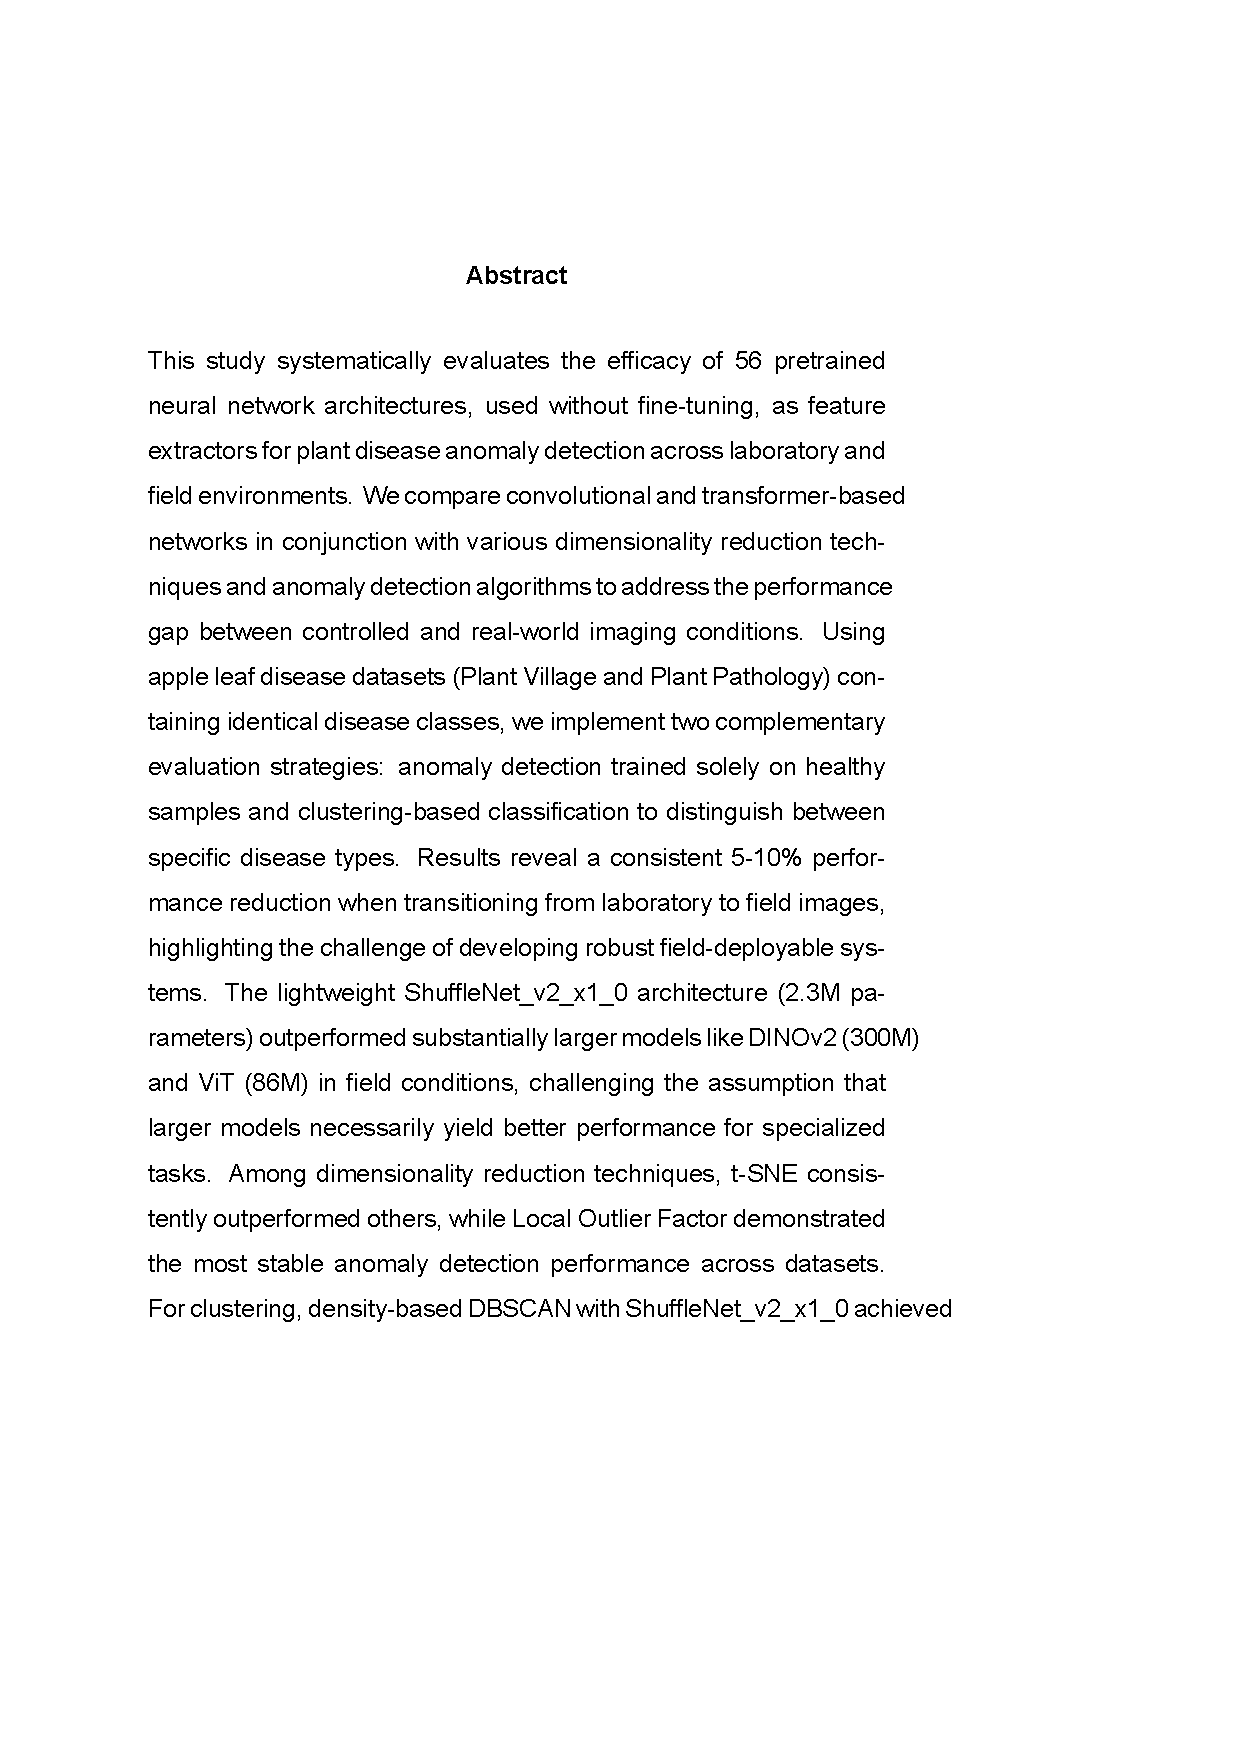
\includepdf[pages=1-7]{Anomaly_detection/Anomaly_detection.pdf}
\includepdf[pages=8,landscape=true]{Anomaly_detection/Anomaly_detection.pdf}
\includepdf[pages=9-]{Anomaly_detection/Anomaly_detection.pdf}


\chapter{Conclusions}

This thesis has systematically investigated the integration of geomatics techniques 
with geostatistical methods to improve PPP efficacy and selectivity evaluations. 
Through a series of complementary case studies, we have demonstrated the feasibility 
and practical requirements for leveraging spatial data to more effectively model 
and exclude environmental variability from statistical analyses.

The first case study established that photogrammetry combined with machine learning 
provides a robust methodology for obtaining spatial coordinates alongside continuous 
variable observations, specifically plant counts. Our research determined precise 
dataset requirements for deploying these technologies within the EPPO framework. 
We found that transformer-mixed architectures (RT-DETR) required fewer training samples 
(approximately 60) to achieve benchmark performance compared to pure CNN models like YOLO 
variants, which needed substantially more samples (110-130). Importantly, we demonstrated that in-domain training 
data is essential for reliable performance, as no out-of-distribution trained model 
achieved the EPPO benchmark regardless of architecture. This finding has significant 
implications for the future of digital data collection in phytosanitary trials, as it
suggests that even with advanced models, the need for domain-specific training data
remains critical for achieving accurate and reliable results.

The second case study (ordinal variables) explored the automation of phytotoxicity scoring using geomatics techniques. The integration of photogrammetric 3D modeling with multispectral imaging enabled accurate reproduction of visual assessments ($\kappa$ > 0.7) while providing precise spatial coordinates for each observation. This geomatic approach not only automated subjective evaluations but also facilitated the conversion of ordinal data to continuous scales, enabling more powerful parametric statistical analyses within geostatistical frameworks.

The third case study (binary and nominal variables) demonstrated the effectiveness of combining pre-trained machine learning models with georeferenced data for plant health classification. The geomatic workflow provided spatial context for anomaly detection algorithms, achieving accuracy > 0.85 without requiring task-specific training data. This approach particularly benefits from the spatial organization of data that geomatics provides, enabling more robust unsupervised learning strategies.

\section{Geomatic Contributions and Innovations}

This research has demonstrated that geomatics techniques provide three critical advantages for PPP trials:

\textbf{Spatial Data Integration:} Photogrammetry and spectral imaging workflows automatically generate precise spatial coordinates alongside observations, eliminating the traditional barrier to implementing geostatistical methods in agricultural trials. Our findings show that centimeter-level accuracy is achievable across all EPPO variable types.

\textbf{Enhanced Data Density:} Geomatics techniques enable collection of thousands of spatially-referenced observations compared to traditional manual methods. This dramatic increase in sample size improves statistical power while maintaining spatial independence through appropriate geostatistical modeling.

\textbf{Reproducibility and Standardization:} Digital geomatics workflows provide objective, repeatable measurements that reduce human bias and improve inter-observer consistency. The georeferenced datasets enable retrospective analysis and validation, supporting regulatory requirements for data quality and traceability.

\section{Future Research Directions}

Several promising avenues emerge from this work:

\textbf{Temporal Geostatistics:} Extending spatial modeling to include temporal dimensions using time-series drone surveys could improve understanding of treatment effects over crop development cycles.

\textbf{Multi-sensor Fusion:} Combining thermal, LiDAR, and hyperspectral data within unified geomatic workflows may enable detection of subtle stress responses currently missed by visual assessments.

\textbf{Real-time Processing:} Developing edge computing solutions for in-field geomatic analysis could enable adaptive trial management and early detection of experimental issues.

\textbf{Regulatory Integration:} Collaborating with EPPO to develop standardized protocols for digital data validation and acceptance within regulatory frameworks.

In conclusion, this thesis establishes geomatics as a transformative technology for PPP evaluation, providing practical solutions to longstanding challenges in agricultural statistics. The integration of spatial data collection with geostatistical analysis represents a paradigm shift toward more robust, objective, and statistically powerful efficacy assessments that better serve agricultural research and regulatory decision-making.


\includepdf[pages=-]{Intestazione/ringraziamenti.pdf}
\end{document}
